% This is samplepaper.tex, a sample chapter demonstrating the
% LLNCS macro package for Springer Computer Science proceedings;
% Version 2.20 of 2017/10/04
%
\documentclass[runningheads]{llncs}
%
\usepackage{graphicx}
\usepackage{multirow} 
\usepackage{fancyvrb}
\usepackage[misc,geometry]{ifsym} 
\usepackage{subcaption}
\usepackage{caption}
\usepackage{listings}
\usepackage{xcolor}
\usepackage{booktabs}
\newcommand{\ra}[1]{\renewcommand{\arraystretch}{#1}}
\setlength{\tabcolsep}{0.7em}

\lstloadlanguages{Python}
\lstset{
  language=Python,
  basicstyle=\scriptsize\sffamily,
  numberstyle=\color{gray},
  stringstyle=\color[HTML]{933797},
  commentstyle=\color[HTML]{228B22}\sffamily,
  emph={[2]from,import,pass,return}, emphstyle={[2]\color[HTML]{DD52F0}},
  emph={[3]range}, emphstyle={[3]\color[HTML]{D17032}},
  emph={[4]for,in,def}, emphstyle={[4]\color{blue}},
  showstringspaces=false,
  breaklines=true,
  prebreak=\mbox{{\color{gray}\tiny$\searrow$}},
  numbers=left,
  xleftmargin=15pt
}

% Used for displaying a sample figure. If possible, figure files should
% be included in EPS format.
%
% If you use the hyperref package, please uncomment the following line
% to display URLs in blue roman font according to Springer's eBook style:
\usepackage{hyperref}
\renewcommand\UrlFont{\color{blue}\rmfamily}

\begin{document}
%
\title{Genegram: RNA Secondary Structure Prediction Using Formal Grammars and Residual Neural Networks\thanks{Supported by the Russian Science Foundation grant 18-11-00100}}
%
\titlerunning{Genegram: CFG + ResNet}
% If the paper title is too long for the running head, you can set
% an abbreviated paper title here
%
\author{Polina Lunina\inst{1,2}\orcidID{0000-0002-7172-2647} \Letter \and
Semyon Grigorev\inst{1,2}\orcidID{0000-0002-7966-0698} \and
Vadim Abzalov\inst{1,2}\orcidID{0000-0002-0805-0315}}
%
\authorrunning{Polina Lunina, Semyon Grigorev, Vadim Abzalov}
% First names are abbreviated in the running head.
% If there are more than two authors, 'et al.' is used.
%
\institute{Saint Petersburg State University, 7/9 Universitetskaya nab., St. Petersburg, 199034, Russia \and
JetBrains Research, Primorskiy prospekt 68-70, Building 1, St. Petersburg 197374, Russia\\
\email{lunina\_polina@mail.ru \Letter, semyon.grigorev@jetbrains.com, vadim.i.abzalov@gmail.com}\\
}
%
\maketitle             % typeset the header of the contribution
%
\begin{abstract}
Improvement in RNA secondary structure prediction accuracy is one of the key focuses in computational genomics due to its crucial role in the functional analysis of RNA molecules. We propose a new approach to solve this problem. Simple context-free grammar describes the most common types of stems and the parsing matrix for some sequence represents all the theoretically possible folds for each subsequence. This information is excessive because only one combination of stems will be presented in a real secondary structure. Moreover, the parsing matrix can be incomplete due to inevitable limitations in grammar. So, we process parsing matrices with residual neural networks in order to generate a valid secondary structure. This approach allows to process pseudoknots, wobble base pairs, and multiple contacts due to the flexible nature of the neural network training process. Our solution was implemented as a Python console tool Genegram.

\keywords{RNA \and Secondary Structure \and Genomic Sequences \and CNN \and ResNet \and Machine Learning  \and Formal Grammars \and Parsing.}
\end{abstract}
%
%
%
\section{Introduction}
\section{Introduction}

Scalable high-performance graph analysis is an actual challenge.
There is a big number of ways to attack this challenge~\cite{Coimbra2021} and the first promising idea is to utilize general-purpose graphic processing units (GPGPU).
Such existing solutions, as CuSha~\cite{10.1145/2600212.2600227} and Gunrock~\cite{7967137} show that utilization of GPUs can improve the performance of graph analysis, moreover it is shown that solutions may be scaled to multi-GPU systems.
But low flexibility and high complexity of API are problems of these solutions.

The second promising thing which provides a user-friendly API for high-performance graph analysis algorithms creation is a GraphBLAS API~\cite{7761646} which provides linear algebra based building blocks to create graph analysis algorithms.
The idea of GraphBLAS is based on a well-known fact that linear algebra operations can be efficiently implemented on parallel hardware.
Along with that, a graph can be natively represented using matrices: adjacency matrix, incidence matrix, etc.
While reference CPU-based implementation of GraphBLAS, SuiteSparse:GraphBLAS~\cite{10.1145/3322125}, demonstrates good performance in real-world tasks, GPU-based implementation is challenging.

One of the challenges in this way is that real data are often sparse, thus underlying matrices and vectors are also sparse, and, as a result, classical dense data structures and respective algorithms are inefficient. 
So, it is necessary to use advanced data structures and procedures to implement sparse linear algebra, but the efficient implementation of them on GPU is hard due to the irregularity of workload and data access patterns.
Though such well-known libraries as cuSPARSE show that sparse linear algebra operations can be efficiently implemented for GPGPU, it is not so trivial to implement GraphBLAS on GPGPU. 
First of all, it requires \textit{generic} sparse linear algebra, thus it is impossible just to reuse existing libraries which are almost all specified for operations over floats.
The second problem is specific optimizations, such as masking fusion, which can not be natively implemented on top of existing kernels.
Nevertheless, there is a number of implementations of GraphBLAS on GPGPU, such as GraphBLAST~\cite{yang2019graphblast}, GBTL~\cite{7529957}, which show that GPGPUs utilization can improve the performance of GraphBLAS-based graph analysis solutions.
But these solutions are not portable because they are based on Nvidia Cuda stack.
Moreover, the scalability problem is not solved: all these solutions support only single-GPU, not multi-GPU computations.

To provide portable GPU implementation of GraphBLAS API we developed a \textit{SPLA} library\footnote{Source code available at: \url{https://github.com/JetBrains-Research/spla}}.
This library utilizes OpenCL for GPGPU computing to be portable across devices of different vendors.
Moreover, it is initially designed to utilize multiple GPGPUs to be scalable.
To sum up, the contribution of this work is the following.
\begin{itemize}
    \item Design of portable GPU GraphBLAS implementation proposed. The design involves the utilization of multiple GPUS. Additionally, the proposed design is aimed to simplify library tuning and wrappers for different high-level platforms and languages creation. 
    \item Subset of GraphBLAS API, including such operations as masking, matrix-matrix multiplication, matrix-matrix e-wise addition, is implemented. The current implementation is limited by COO and CSR matrix representation format and uses basic algorithms for some operations, but work in progress and more data formats will be supported and advanced algorithms will be implemented in the future.
    \item Preliminary evaluation on such algorithms as breadth-first search (BFS) and triangles counting (TC), and real-world graphs shows portability across different vendors and promising performance: for some problems Spla is comparable with GraphBLAST. Surprisingly, for some problems, the proposed solution on embedded Intel graphic card shows better performance than SuiteSparse:GraphBLAS on the respective CPU. At the same time, the evaluation shows that further optimization is required.
\end{itemize} 

\section{Proposed Approach Overview}
In this section, we focus more on the theoretical aspects of the proposed approach that underlie the experimental research presented in section 3. 

Secondary structure can be viewed as a recursive composition of stems having different lengths and loop sizes~\cite{MQbioinformatics19}, so, we propose to use formal grammar to encode the most common types of stems, considering RNA sequence as a string in the $\{A, C, G, U\}$ alphabet. Thereby, the parsing matrix for some sequence will contain information about whether each subsequence of this sequence can fold to stem or not. This matrix is not yet a representation of a valid secondary structure, because all these stems cannot exist at once and, besides, there can be more complex elements that are not expressible in terms of given grammar (for example, pseudoknots and wobble base pairs). Therefore, we propose to process parsing matrices by neural networks that should filter extra stems and add the missing elements in order to generate a maximal approximation of real secondary structure in some compatible with another studies format. In figure~\ref{arch} the global solution architecture is presented and in the next sections, we will speak in detail about each of the specified components.

\begin{figure}[h]
\centering
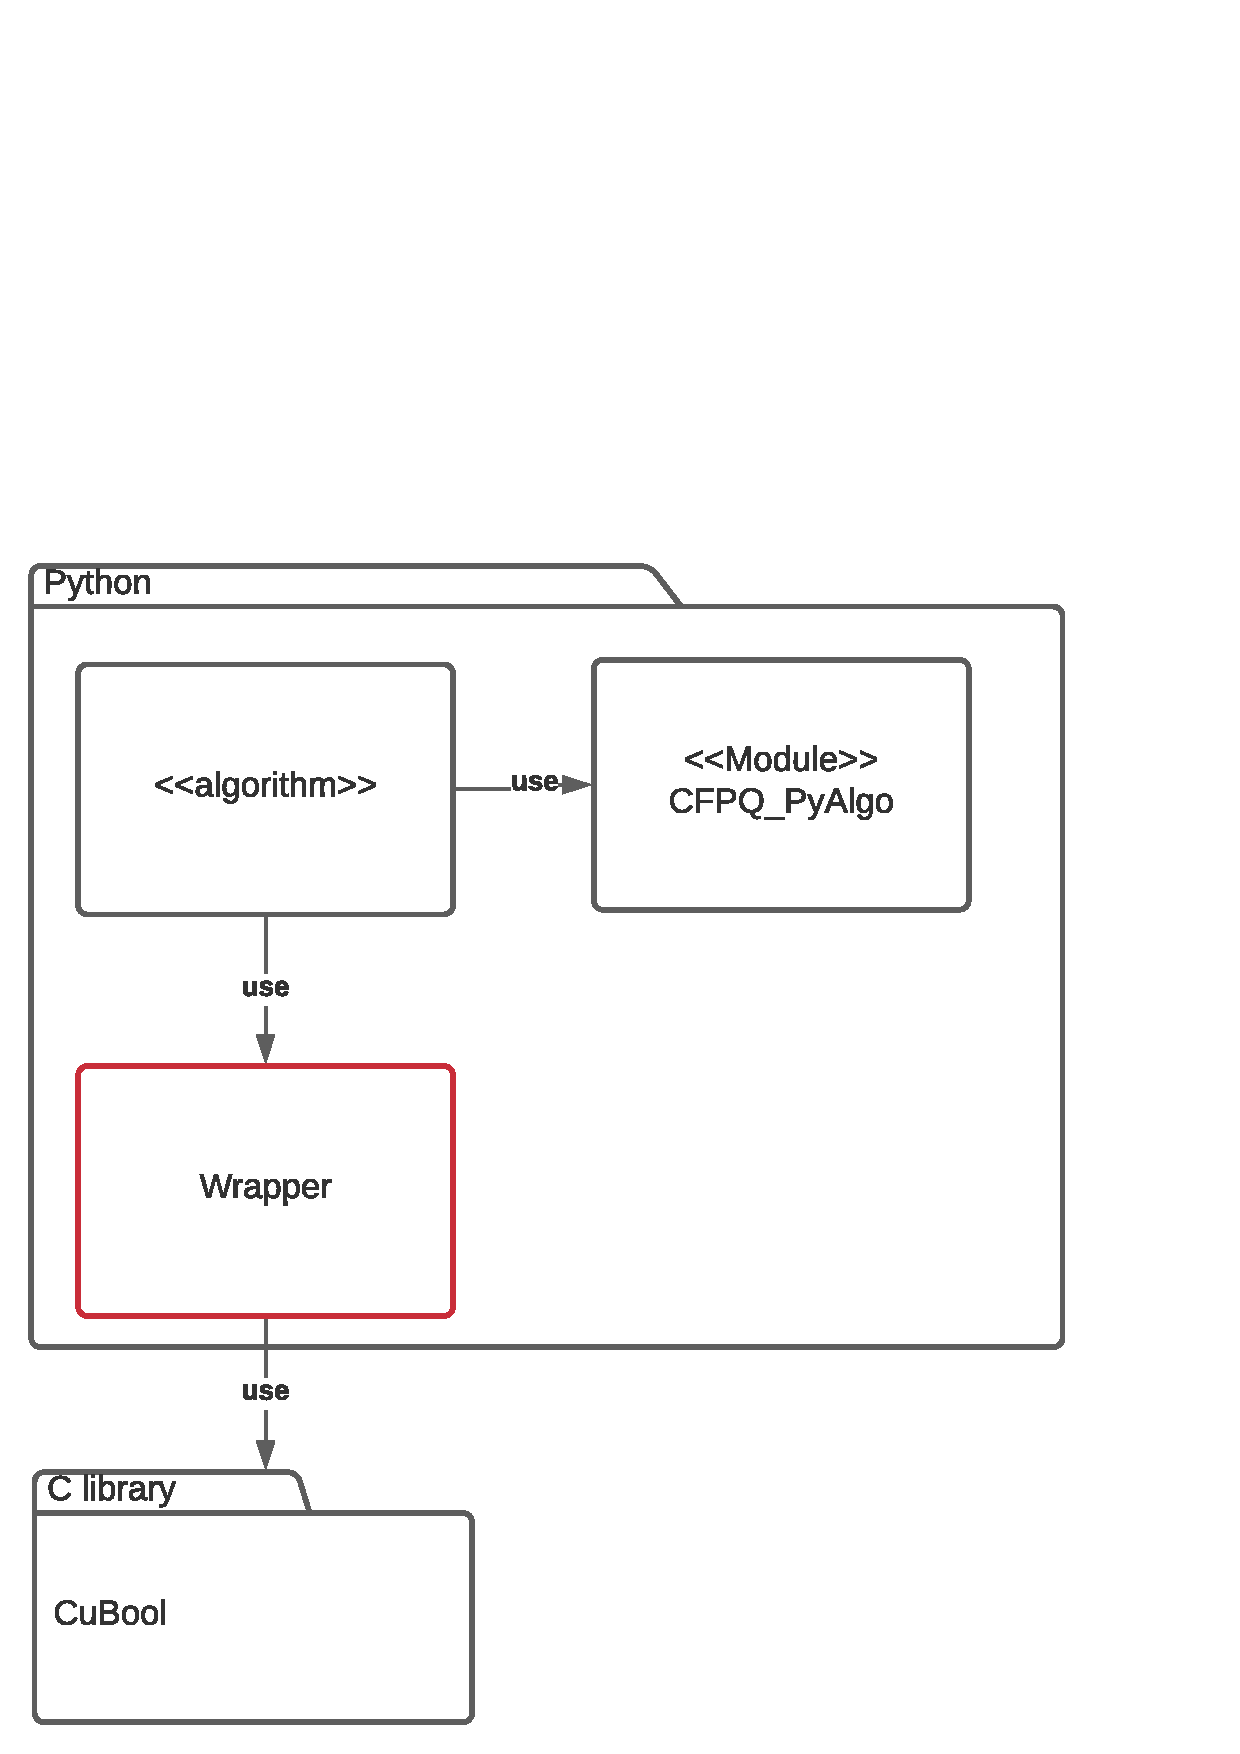
\includegraphics[width=\textwidth]{pics/arch.pdf}
\caption{Global solution architecture}
\label{arch}
\end{figure}

\subsection{Formal Grammar}
As it was mentioned before, our approach employs formal grammar not for modeling the whole structure, but for encoding its simple constructional elements (stems), therefore this grammar does not require probabilistic rules --- probability estimation is to be done by neural networks. We do not strictly fix the grammar and it can be modified in accordance with research purposes or data characteristics, so, the grammar presented below is just a concrete example that showed quite successful results during the experiments.

In figure~\ref{gram} context-free grammar $G_0$ that we use in this work as well as in the previous ones is presented. This grammar describes the recursive compositions of stems having height at least 3 (lines \textbf{7-12}) and loop size from 1 up to 20 (line \textbf{3}). Note that these constants are not mandatory and might be defined experimentally for each task. Also, $G_0$ allows only four classical nucleotides (line \textbf{4}) and conventional base pairs (line \textbf{5}), because adding the rules for more pairs and nucleotides complicates the grammar unacceptably in the context of performance, moreover, context-free grammars cannot explicitly express pseudoknots, therefore, we expect the neural network to handle all these features instead. Also, we consider only stems of height three or more (lines \textbf{1-2}), because including shorter stems would overload the parsing matrix with too much extra information. So, by this rules, a sequence folds to stem if and only if it is derivable from start nonterminal $start$ of $G_0$ (line \textbf{1}).

\begin{figure}[ht]
\begin{Verbatim}[numbers=left,xleftmargin=5mm]
start: stem3<s0>
s0: loop | loop stem3<s0> s0
loop: nucl*[1..20]
nucl: A | U | C | G
stem1<s>: A s U | G s C | U s A | C s G
stem2<s>: stem1<stem1<s>>
stem3<s>: 
      stem1<stem2<s>>
    | A stem3<s> U
    | U stem3<s> A
    | C stem3<s> G
    | G stem3<s> C
\end{Verbatim}
\caption{Context-free grammar $G_0$ for RNA secondary structure stems description}
\label{gram}
\end{figure}

Having a grammar, we want to find all the subsequences of some given sequence that may fold to stems and this is to be done by means of parsing. Formally, the result of a matrix-based parsing algorithm for an input string $w$ is an upper-triangular boolean matrix $M_P$, where $M_P [i,j] = 1$ if and only if the substring $w[i,j]$ is derivable from grammar start nonterminal. From the practical point of view, this means that parsing matrix contains one in a cell if and only if a correspondent substring folds to stem according to the rules of a given grammar, so, each stem results in a diagonal chain of ones in the matrix, because if sequence $w_1...w_n$ is a stem than it is clear that $w_2...w_{n - 1}$ is a stem, $w_3...w_{n - 2}$ is a stem and so on while the stem height is at least 3.

In figure~\ref{pars_res} we provide the parsing result for a short RNA sequence and show how parsing matrix maps with secondary structure stems. Each one cell describes the stem of height at least 3, so, this sequence contains two subsequences that may fold to stems of the first nesting level. These stems expected hydrogen bonds along with corresponding matrix cells are painted in two different colors. All nucleotide bonds forming a stem of height three or more are represented by solid lines, moreover, it is obvious that each stem of height three encapsulates stems of heights two and one which are highlighted by dotted lines. Note that these stems interfere with each other, thereby, secondary structure cannot contain both of them at the same time. So, the parsing matrix for a sequence describes all the theoretically possible folds there, but at the current step, we cannot know which one of them would be presented in the real secondary structure. Moreover, $G_0$ has certain limitations, such as stem height, loop size, and possible base pairs, so, some of the required stems may be missing in the parsing matrix. While creating a grammar we were guided by two competing ideas: to cover as many types of stems as possible and to stay with an adequate amount of extra information in the parsing matrix along with acceptable time costs for parsing.

\begin{figure}[h]
\centering
\valign{#\cr
  \hbox{%
    \begin{subfigure}[b]{.6\textwidth}
    \centering
    \includegraphics[width=\textwidth]{pics/matrix.pdf}
    \caption{Parsing matrix}
    \label{mtrx}
    \end{subfigure}%
  }\cr
  \noalign{\hfill}
  \hbox{%
    \begin{subfigure}{.4\textwidth}
    \centering
    \vspace{2mm}
    \includegraphics[width=.3\textwidth]{pics/stem1.pdf}
    \caption{First stem}
    \label{stem1}
    \end{subfigure}%
  }\vfill
  \hbox{%
    \begin{subfigure}{.4\textwidth}
    \centering
     \vspace{-2mm}
    \includegraphics[width=.3\textwidth]{pics/stem2.pdf}
    \caption{Second stem}
    \label{stem2}
    \end{subfigure}%
  }\cr
}
\caption{Stems extracted from RNA sequence by parser}
\label{pars_res}
\end{figure}

Let us consider pseudoknotted structures processing. Even though it is clear that pseudoknot is not explicitly expressed in $G-0$, as well as in any context-free grammar, it consists of two stem-loop structures having half of one stem located between two halves of another, so, each of these stems separately can be derived by the rules of $G_0$. Therefore, pseudoknots will be reflected in the parsing matrix, and handling them becomes an additional task for a neural network. In figure~\ref{pk} an example of simple pseudoknot along with corresponding parsing result is provided. Two stems of this pseudoknot are highlighted with two different colors and it can be seen that all the related nucleotide bonds are presented in the parsing matrix, although at this point it is not determined whether this sequence contains a pseudoknot or it just has two possible folds in terms of grammar.

\begin{figure}[h]
\centering
\begin{subfigure}{.3\textwidth}
  \centering
  \hbox{\includegraphics[width=.9\linewidth]{pics/pk.pdf}}
  \caption{Pseudonkot}
  \label{pk_a}
\end{subfigure}%
\begin{subfigure}{.7\textwidth}
  \centering
  \hbox{\includegraphics[width=.9\linewidth]{pics/matrix_pk.pdf}}
  \caption{Parsing matrix}
  \label{pk_b}
\end{subfigure}
\caption{Pseudoknots processing in terms of $G_0$}
\label{pk}
\end{figure}

To sum up, our grammar explicitly or implicitly describes a wide range of secondary structure elements and even the missing ones do not become a problem for our approach --- neural network is still capable to handle them. We think of such flexibility as one of the key advantages of our solution.

\subsection{Neural Network}
The matrix that our parser produced for some sequence and fixed grammar should be processed by a neural network in order to achieve a maximal similarity with the expected secondary structure for this sequence. Therefore, we need to specify the data preparing pipeline and describe the required architecture for the problem at hand. It should be noted that these are global and permanent aspects in the context of current work, however, both of them can and probably will be changed while conducting some different research.

\subsubsection{Data}
The input data for neural network (parsing matrices) was described in the previous section and now let us define the reference data source and format. There are specialized biological databases containing RNA chains of various organisms along with their secondary structures obtained by reliable methods, and such data is known to be the best for algorithms training and validation. These databases may store data using different representations (dot-bracket, connectivity table, and others), so, we need to choose a format that is convenient for our experiments and compatible with others.

One of the ways of RNA secondary structure formal representation is so-called contact map, which for an input string $w$ is a boolean matrix $M_C$, where $M_C [i,j] = 1$ if and only if nucleotides in positions $i$ and $j$ form a hydrogen bond (or, to put it simply, a contact) in secondary structure. Even though it is not the most popular format, contact matrix can be easily obtained from the corresponding connectivity table, moreover, there are certain tools that transform connectivity tables to dot-brackets~\cite{bellaousov2013rnastructure}, which provides the required compatibility. Let us consider for the above sequence $w$ the discussed earlier parsing matrix $M_P$ that has $M_P[i, j] = 1$ if and only ifsubsequence $w[i, j]$ folds to a stem. It is clear that the first and the last nucleotides of every stem form a contact, therefore, we can easily transfer between parsing matrix and contact map definitions and view the parsing matrix as a sort of a contact map, so, this format is convenient for our experiments. Note that if parser finds a stem of height three than we will see only one cell with $1$ in matrix, but such stem always wraps a stem of height two which wraps a stem of height one, so, we are always missing two contacts, therefore, after parsing we should set $M_P[i - 1, j + 1] := 1$ , $M_P[i - 2, j + 2] := 1$ if $M_P[i][j] = 1$, $i = 0..size(M_P), j = i + 1..size(M_P)$ for complete semantic equality of parsing and contact matrices.

So, a neural network should take parsing matrices as inputs and contact maps as desired outputs for the same set of RNA sequences. For convenience, we transform both matrices to black-and-white images by replacing zero cells with black pixels and one cells with white pixels. Also, we code RNA sequence at the input image main diagonal by four types of gray pixels corresponding to the four possible nucleotides in case the chain itself contains any important information about secondary structure formation patterns.

In figure~\ref{struc} we provide two-dimensional secondary structure visualization for RNA sequence along with neural network input and reference images that were made from parsing and contact matrices respectively. Contacts belonging to the three stems presented in this sequence are highlighted with three different colors in all pictures (so, input and reference images are actually grayscale, colored pixels are only here for clarification). It can be seen that not all of the stems found by the parser are presented in the real secondary structure. Moreover, the parsing result is missing several contacts since they were formed by non-canonical nucleotide pairs $A-G$ that are not expressed by grammar $G_0$. Now the purpose of a neural network becomes clear --- it should take image~\ref{struc_b} and transform it to the image~\ref{struc_c} as accurately as possible. And the ideas behind this transformation are outlined in the next section.

\captionsetup[subfigure]{justification=centering}
\begin{figure}[h]
\centering
\begin{subfigure}{.33\textwidth}
  \centering
  \hbox{\includegraphics[width=\linewidth]{pics/struct.pdf}}
  \caption{Secondary structure visualization}
  \label{struc_a}
\end{subfigure}%
\begin{subfigure}{.33\textwidth}
  \centering
  \hbox{\includegraphics[width=\linewidth]{pics/in.png}}
  \caption{Input image \\ for neural network}
  \label{struc_b}
\end{subfigure}
\begin{subfigure}{.33\textwidth}
  \centering
  \hbox{\includegraphics[width=\linewidth]{pics/out.png}}
  \caption{Reference image \\ for neural network}
  \label{struc_c}
\end{subfigure}
\caption{Secondary structure representations}
\label{struc}
\end{figure}

\subsubsection{Parallel ResNet}
One of the popular architectures for complicated images processing tasks is a residual neural network based on adding skip connections between blocks of layers~\cite{he2016deep}. ResNets solve the problem of vanishing gradient and allow to effectively use deep convolutional networks.

In this work, we developed a new architecture that showed its applicability for secondary structure prediction task during experimental research. The idea is to combine $n$ identical residual networks that take the same input, go through independent sequences of layers and connect their $n$ outputs with weighted sum hanging it over to the final residual unit that directly generates output. This parallel residual architecture along with the scheme of a typical residual unit is presented in figure~\ref{nn}, where $k$ and $n$ can be selected based on empirical evidence. We believe that the advantage of this parallel technique is that these separate networks are able to find different types of features in data and some sort of voting system allows the whole model to decide for the particular pixel whether each network behaves correctly or not.

\begin{figure}[h]
\centering
\includegraphics[width=\linewidth]{pics/nn.pdf}
\caption{Parallel ResNet architecture}
\label{nn}
\end{figure} 

\section{Experiments}
Для экспериментальных исследований были необходимы данные двух типов: последовательности РНК для подачи на вход синтаксическому анализатору и эталонные вторичные структуры для этих последовательностей --- и то, и другое было получено из популярной в исследовательских работах базы данных RNAstrand~\cite{andronescu2008rna}. Эта база представляет собой сборку тщательно отобранных и приведенных к единому формату данных сразу из нескольких надежных баз, содержащих цепочки РНК вместе с полученными методами лабораторного эксперимента или эволюционного анализа вторичными структурами. Из выгруженных данных были удалены дубликаты и образцы с неточностями в нуклеотидной цепи или же вторичной структуре, а также было выставлено ограничение на максимальную длину последовательности --- таким образом была получена выборка из 801 последовательности длин от 8 до 100, для которой были сгенерированы матрицы разбора и матрицы контактов, переведенные в черно-белые изображения. Для цепочки длины $n$ и входное, и эталонное изображения имеют размер $n \times n$, поэтому для корректной обработки изображений разного размера перед каждой эпохой обучения нейросети данные группировались по батчам, в каждом из которых присутствовали изображения только одного размера. Распределение длин последовательностей в итоговой выборке продемонстрировано на рис.~\ref{plot_distr}, при этом медианным значением является 44, а средним --- 47, что говорит о практически одинаковой представленности коротких и длинных цепочек среди исследуемых данных.

\begin{figure}[h]
\begin{center}
\centering
\includegraphics[width=16cm]{pics/plot_distr.png}
\caption{Распределение длин последовательностей РНК в выборке}
\label{plot_distr}
\end{center}
\end{figure} 

Для оценки качества работы обученных на данных изображениях нейронных сетей были выбраны следующие метрики, посчитанные относительно попиксельной разницы между предсказанным и эталонным изображениями. Далее $TP$ (true positive), $FP$ (false positive) и $FN$ (false negative), где под positive и negative  понимаются белые и черные пиксели изображений соответственно, --- информация о том, сколько раз нейронная сеть приняла верное и сколько раз неверное решение по каждому пикселю (кроме диагональных) каждого изображения тестовой выборки.
\begin{itemize} 
    \item $Precision = \frac{TP}{TP + FP}$ (доля предсказанных контактов, которые действительно являются контактами в эталонном изображении).
    \item $Recall = \frac{TP}{TP + FN}$ (доля найденных нейронной сетью контактов среди всех искомых).
    \item $F1 = 2 * \frac{Precision * Recall}{Precision + Recall}$ (гармоническое среднее $Precision$ и $Recall$, используется как удобная объединяющая метрика).
\end{itemize}

При обучении нейросети была использована функция потерь, в основе построения которой лежит идея о максимизации метрики $F1$ с несколькими уточнениями. Во-первых, $F1$ дискретна, а функция ошибки должна быть дифференцируема вследствие вычисления на ней градиента. Во-вторых, передача среднего по выборке значения $1 - F1$ в качестве функции ошибки не гарантирует отсутствие большого разброса $Precision$ и $Recall$ как в пределах отдельно взятого изображения, так и в масштабах всей выборки, следствием чего будет нестабильность качества работы модели и высокая вероятность появления очень низкой точности результата для случайно взятого тестового образца. На основании данных соображений была реализована функция $F1\_loss$, представленная на рис.~\ref{loss}. Здесь дифференцируемость обеспечивается заменой сумм дискретных целочисленных значений на непрерывную сумму значений вероятности, а поддержка баланса между $Precision$ и $Recall$ для каждого изображения и для выборки в целом --- двумя пропорциональными величине разброса штрафными коэффициентами $k1$ и $k2$, накладываемыми на метрику $F1$.

\begin{figure}[h]
\begin{center}
\centering
\begin{python}
from keras import backend as K

def f1_loss(y_true, y_pred):
    #normalize pixels values to [0, 1]
    y_true, y_pred = K.minimum(y_true / 255, 1), K.minimum(y_pred / 255, 1)
    #calculate differentiable versions of TW, FW and FB
    tw = K.sum(K.cast(y_true * y_pred, 'float32'), axis=[1, 2, 3])
    fw = K.sum(K.cast((1 - y_true) * y_pred, 'float32'), axis=[1, 2, 3])
    fb = K.sum(K.cast(y_true * (1 - y_pred), 'float32'), axis=[1, 2, 3])
    #calculate precision and recall secure from zero division error
    precision = tw / (tw + fw + K.epsilon())
    recall = tw / (tw + fb + K.epsilon())
    #penalty coefficients for huge difference between precision and recall 
    #calculated for each image and whole dataset respectively
    k1 = 1 -  K.abs(precision - recall)
    k2 = 1 -  K.abs(K.mean(precision) - K.mean(recall))
    #calculate upgraded f1 score
    f1 = k1 * k2 * 2 * precision * recall / (precision + recall + K.epsilon()) 
    return 1 - K.mean(f1)
\end{python}
\caption{Функция потерь нейронной сети}
\label{loss}
\end{center}
\end{figure} 

Вследствие того, что количество обучаемых параметром используемой модели является достаточно большим относительно размера обучающей выборки, после каждого остаточного блока был добавлен слой Dropout, исключающий заданный процент случайных нейронов во время обучения. Кроме того, во всех сверточных слоях была применена регуляризация L2, которая, помимо уменьшения переобучения нейросети, оказывает положительное влияние на процесс поиска сложных закономерностей в данных. В качестве оптимизатора был использован адаптивный градиентный спуск (Adagrad)~\cite{duchi2011adaptive}, удобный для работы с разреженными данными, а также автоматически настраивающий скорость обучения.

Для сравнения результатов работы обученной модели с существующими в области аналогами был проведен анализ различных инструментов, предсказывающих вторичную структуру РНК, по следующим критериям: заявленная высокая точность результатов, возможность предсказания псевдоузлов, удобство использования и адекватное время работы. На основании данных соображений были отобраны шесть инструментов, основанных на различных подходах.
\begin{itemize}
    \item HotKnots --- минимизации свободной энергии через эвристический алгоритм~\cite{ren2005hotknots}.
    \item SPOT-RNA --- глубокое обучение, основанное на технике transfer learning~\cite{singh2019rna}.
    \item PknotsRG --- минимизация свободной энергии с использованием Turner energy rules~\cite{reeder2007pknotsrg}.
    \item RNAstructure --- минимизация свободной энергии с помощью динамического программирования~\cite{bellaousov2013rnastructure}.
    \item Ipknot --- поиск оптимальной вторичной структуры методом целочисленного программирования~\cite{sato2011ipknot}.
    \item Knotty --- алгоритм для минимизация свободной энергии, основанный на разреженном динамическом программировании~\cite{jabbari2018knotty}.
\end{itemize}

\subsection{Результаты}
Все тестовые запуски проводились на рабочей станции со следующими характеристиками.
\begin{itemize}
    \item Операционная система: Ubuntu 20.04.2 LTS.
    \item Центральный процессор: Intel Core i5-10210U CPU 1.60GHz.
    \item Графический процессор: NVIDIA GeForce MX250.
    \item Объем оперативной памяти: 7.5 GB.
\end{itemize}

На рис.~\ref{plot_f1} представлены значения метрики $F1$, показанные шестью вышеописанными инструментами на всей выборке из 801 образца, а разработанной моделью (New-model) --- для различных разделений данных на обучающую и тестовую выборки (10\%:90\%, ..., 90\%:10\%). На графике видно, что при малых размерах обучающей выборки новая модель демонстрирует достаточно низкую точность, однако при увеличении выборки до 40\% результаты становятся сравнимыми с остальными подходами, а при максимальном объеме выборки (90\%) ---  лучшими в приведенном сравнении.

На рис.~\ref{plot_pr} показаны результаты аналогичного тестирования всех моделей по метрикам $Precision$ и $Recall$; здесь черная прямая $y=x$ символизирует оптимальное для рассматриваемой задачи положение этих метрик --- их равенство, --- а фиолетовая пунктирная линия указывает направление увеличения размера обучающей выборки для нашей модели от 10\% до 90\% с шагом в 10\%. Значения метрик для New-model расположены достаточно близко к желаемой прямой, что говорит о сбалансированности предсказаний разработанной нейросети. Кроме того, реализованный в данной работе алгоритм --- единственный на данном графике, имеющий $Recall$, больший, чем $Precision$: это произошло из-за того, что парсер находит значительную часть требуемых контактов, поэтому нейронная сеть, владея этой информацией еще до начала обучения, основной своей задачей имеет улучшение точности, а не полноты системы. Это делает наш подход несколько нетрадиционным относительно аналогов, которые, по всей видимости, сталкиваются с рядом проблем в процессе поиска контактов во вторичной структуре.

\begin{figure}[h]
\centering
\begin{subfigure}{.5\textwidth}
  \centering
  \fbox{\includegraphics[width=.95\linewidth]{pics/plot_f1.png}}
  \caption{Значения метрики $F1$}
  \label{plot_f1}
\end{subfigure}%
\begin{subfigure}{.5\textwidth}
  \centering
  \fbox{\includegraphics[width=.95\linewidth]{pics/plot_pr.png}}
  \caption{Значения метрик $Precision$ и $Recall$}
  \label{plot_pr}
\end{subfigure}
\caption{Сравнение разработанного подхода с аналогами}
\label{plot}
\end{figure}

Помимо точности, важной характеристикой алгоритма в области биоинформатики является время его работы, так как исследователям часто приходится работать с достаточно большими биологическими базами данных. В таблице~\ref{time} приведены замеры времени, потраченного всеми инструментами на обработку 100 цепочек РНК различных длин из рассматриваемого промежутка от 8 до 100. Несмотря на то, что разные подходы могут предполагать разные сценарии использования (обработка одной или нескольких последовательностей, вывод ответа через интерфейс командной строки или в специальный файл, а также сохранение результатов в различных форматах), одним из традиционных вариантов является обработка файла в формате fasta, содержащего набор последовательностей с метаданными, и последующее сохранение результата в одном из общепринятых форматов (например, dot-bracket или bpseq). Для данного сценария и был произведен сравнительный анализ производительности подходов: файл с последовательности был преобразован в необходимые для всех инструментов входные форматы, выходные же форматы были оставлены без изменений. В таблице~\ref{time} представлены средние значения для десяти прогонов в секундах, упорядоченные по возрастанию времени. Инструменты Ipknot, Hotknots, PknotsRG, RNAstructure и Knotty работают только на CPU, SPOT-RNA имеет и CPU, и GPU-реализации, а для нашего подхода как алгоритм синтаксического анализа (PA), так и нейронная сеть (NN) используют GPU. Можно увидеть, что New-model значительно проигрывает по времени большинству аналогов и наиболее времязатратной операцией здесь является синтаксический анализ, занимающий почти 80\% от общего времени работы.

\begin{table}[]
\centering
\caption{Time measurements for 100 sequences processing}
\begin{tabular}{|p{2cm}||p{2cm}|p{2cm}|p{2cm}|p{2cm}|}
\hline
\multirow{2}{*}{Step} & \multicolumn{2}{l|}{Vector based approach} & \multicolumn{2}{l|}{Image based approach} \\ \cline{2-5} 
 & \begin{tabular}[c]{@{}l@{}}Base \end{tabular} & \begin{tabular}[c]{@{}l@{}}Extended \end{tabular} & \begin{tabular}[c]{@{}l@{}}Base \end{tabular} & \begin{tabular}[c]{@{}l@{}}Extended \end{tabular} \\ \hline \hline
Parse & 307.6s & --- & 310.5s & --- \\ \hline
Load weights & 0.2s & 0.2s & 0.1s & 0.3s \\ \hline
Predict class & 0.2s & 0.2s & 0.2s & 0.3s \\ \hline
Total & 308.0s & 0.4s & 310.8s & 0.6s \\ \hline
\end{tabular}
\label{time}
\end{table}

Подводя итоги, экспериментальные исследования показали работоспособность разработанного подхода применительно к задаче предсказания вторичной структуры РНК даже в сравнении с лучшими инструментами в области. Высокая точность уже полученных результатов вместе с общей гибкостью подхода и обширными возможностями для дальнейших экспериментов позволяют полагать, что предложенные в данной работе идеи имеют значительный потенциал. Однако на данный момент наш проект по большей части исследовательский --- для создания полноценного инструмента требуется тщательный анализ качества всех обученных на различного размера выборках моделей с целью выбора оптимальной, а также, несомненно, повышение производительности подхода, в частности, ускорение синтаксического анализатора.

\section{Conclusion}
\section{Conclusion and Future Work}

We present !!!

Our evaluation shows that !!!

First direction for future research is a more detailed CFPQ algorithms investigation.
We should do More evaluation on sparse matrices on GPGPUs.

Also it is nesessary to implement and evaluate solutions for graphs which is not fit in RAM.
There is a set of technics for huge matrices multiplication.
Is it possible to dopt it for CFPQ

Another direcion is a dataset improvement.
More data.
More grammars/queries.


%
\bibliography{main} 
\bibliographystyle{ieeetr}
\end{document}
